% SoCG 2027 submission draft (Track T: Mathematical Foundations; Algorithmic Complexity).
% Compile with: latexmk -pdf main.tex
%
% CLASS: SoCG requires socg-lipics-v2021.cls (a thin wrapper around lipics-v2021.cls that is
% distributed with the SoCG call for papers). Until the 2027 call is posted we compile with the
% LIPIcs class itself; replace the \documentclass line below by
%   \documentclass[a4paper,USenglish,cleveref,autoref,thm-restate,anonymous]{socg-lipics-v2021}
% once the SoCG wrapper is available, and re-check the line count.
%
% GLOSSARY (one name per object; use these everywhere)
%   norm \|.\|, unit circle S = {x : \|x\| = 1}; Euclidean norm unless stated otherwise
%   G(P)        unit-distance graph of a finite point set P
%   \deg_P(p)   degree of p in G(P);  U(P) = |E(G(P))|  (number of unit-distance pairs)
%   \cP_n       finite point sets with at most n points (n is public)
%   S_k(P)      sum of the k largest degrees of G(P), padded with zeros
%   \Lambda_k(n) top-degree mass = max { S_k(P) : P in \cP_n }
%   I(n,k)      maximum number of incidences between at most n points and k distinct unit circles
%   u(n)        maximum of U(P) over |P| = n
%   tail_D(P)   degree tail = sum_p (\deg_P(p) - D)_+
%   g_D         bounded-degree surrogate (KNRS flow value = fractional b-matching value)
%   err^*(eps,n) minimax expected error of eps-node-private counting over \cP_n
%   "node neighbours": point sets that differ in exactly one point
%
% TODO(authors): the visible "Use of generative AI" paragraph before the bibliography follows the
%   Dagstuhl Publishing GenAI statement (LIPIcs): substantive use must be disclosed in the manuscript
%   (e.g. acknowledgments or before the references) with type, purpose and extent of human review.
%   Do NOT move it into \acknowledgements: the anonymous option hides that field from reviewers.
%   Complete the red sentence truthfully and re-check against the SoCG 2027 call. Strip all
%   comments (including this one) before posting the source to arXiv.
%
% WORDS NOT TO USE: lesson, honest, canonical, load-bearing, operating scale, high-signal,
%   many-distance-pair, promise-oblivious, extremal context, we park, "et al."

\documentclass[a4paper,USenglish,cleveref,autoref,thm-restate,anonymous]{lipics-v2021}

\usepackage{amsmath,amssymb,mathtools}
\usepackage{booktabs}
\usepackage{tikz}

\bibliographystyle{plainurl}

\newcommand{\R}{\mathbb{R}}
\newcommand{\Z}{\mathbb{Z}}
\newcommand{\eps}{\varepsilon}
\newcommand{\cP}{\mathcal{P}}
\newcommand{\cF}{\mathcal{F}}
\newcommand{\Lam}{\Lambda}
\newcommand{\tail}{\operatorname{tail}}
\newcommand{\Lap}{\operatorname{Lap}}
\newcommand{\errs}{\operatorname{err}^*}
\newcommand{\Ex}{\mathbb{E}}
\newcommand{\nrm}[1]{\lVert #1\rVert}

\title{The Top-Degree Mass of Unit-Distance Graphs and the Price of Node Privacy}
\titlerunning{Top-Degree Mass and Node Privacy}

\author{Anonymous author(s)}{Anonymous affiliation}{}{}{}
\authorrunning{Anonymous author(s)}
\Copyright{Anonymous author(s)}

\ccsdesc[500]{Theory of computation~Computational geometry}
\ccsdesc[300]{Security and privacy~Data anonymization and sanitization}
\ccsdesc[300]{Mathematics of computing~Combinatorics}

\keywords{unit distances, incidences, normed planes, differential privacy, node privacy}

\EventEditors{}
\EventNoEds{0}
\EventLongTitle{}
\EventShortTitle{}
\EventAcronym{}
\EventYear{}
\EventDate{}
\EventLocation{}
\EventLogo{}
\SeriesVolume{}
\ArticleNo{}

\begin{document}

\maketitle

\begin{abstract}
Erd\H{o}s asked how many pairs among $n$ points in the plane can be at distance exactly~$1$. We study an unbalanced version of this question and show that it determines the cost of a basic task in data privacy. Let $\Lam_k(n)$ be the largest possible sum of the $k$ largest degrees in the unit-distance graph of at most $n$ points. We prove that the smallest expected error with which the number of unit-distance pairs can be released under $\eps$-node differential privacy is $\Theta(\Lam_{\lceil 1/\eps\rceil}(n))$, with absolute constants, for every $\eps\in(0,1]$. We also show that for $k\le n/2$, $\Lam_k(n)$ equals, up to a factor of~$2$, the maximum number of incidences between $n$ points and $k$ unit circles with arbitrary centres.
We then compare norms on the plane. $\Lam_k(n)=\Theta(kn)$ if the unit circle contains a segment; $\Lam_k(n)=O(n^{2/3}k^{2/3}+n)$ if the norm is strictly convex, and a norm found by Valtr attains this bound for every~$k$; by a theorem of Alon, Buci\'c and Sauermann, $\Lam_k(n)=\Theta(n)$ up to a logarithmic factor for all norms outside a meagre set. For the Euclidean norm the optimal error is $\Theta(n)$ when $\eps\ge n^{-1/2}$, a factor $1/\eps$ below the standard Laplace mechanism. It is polynomially larger than for these generic norms if and only if Erd\H{o}s's unit-distance conjecture fails, which was shown in 2026. Between these ranges the Euclidean question is an open problem on unbalanced unit-circle incidences.
\end{abstract}

%======================================================================
\section{Introduction}
\label{sec:intro}

Let $P$ be a finite set of points in the plane and let $G(P)$ be its \emph{unit-distance graph}: two points are adjacent if their distance is exactly~$1$. Erd\H{o}s~\cite{Erdos46} asked for the maximum number $u(n)$ of edges of $G(P)$ over $n$-point sets. The upper bound $u(n)=O(n^{4/3})$ of Spencer, Szemer\'edi and Trotter~\cite{SpencerSzemerediTrotter84} has not been improved. Erd\H{o}s conjectured $u(n)=n^{1+o(1)}$; in 2026 this conjecture was disproved~\cite{OpenAI2026,Remarks2026}, and Sawin~\cite{Sawin2026} gave sets with more than $n^{1.014}$ unit distances for arbitrarily large~$n$.

This paper studies a refinement of $u(n)$ that measures how unevenly unit distances can be distributed among the points. For a finite set $P$ and an integer $k\ge1$, let $S_k(P)$ be the sum of the $k$ largest degrees of $G(P)$ (padded with zeros if $k>|P|$), and define the \emph{top-degree mass}
\[
  \Lam_k(n)\;=\;\max\{S_k(P): |P|\le n\}.
\]
In this definition the $k$ points whose degrees are summed belong to $P$; the maximum is over all sets of at most $n$ distinct points. Thus $\Lam_1(n)=n-1$ for $n\ge2$ (a point together with $n-1$ points on its unit circle), and $\Lam_k(n)=2u(n)$ for $k\ge n$. In between, $\Lam_k(n)$ asks how many unit distances $k$ points can see.

\subparagraph*{The privacy problem.}
Our motivation comes from differential privacy. Suppose each point of $P$ is the location of one person, and we wish to publish the number $U(P)$ of unit-distance pairs. \emph{Node differential privacy} requires that adding or removing one person, together with all pairs that contain this person, changes the distribution of the published value by at most a factor $e^{\eps}$ (see \cref{sec:prelim} for a self-contained introduction). One point can form a unit-distance pair with all others, so the standard Laplace mechanism must add noise of order $n/\eps$. We ask for the \emph{minimax error}
\[
  \errs(\eps,n)\;=\;\inf_{M}\ \sup_{|P|\le n}\ \Ex\,\bigl|M(P)-U(P)\bigr|,
\]
where $M$ ranges over $\eps$-node-private algorithms and $n$ is a public bound on the number of points. Our first result says that, up to constant factors, this privacy question is the geometric question above.

\begin{restatable}[Reduction]{theorem}{reduction}
\label{thm:reduction}
For every norm on $\R^2$, every $n\ge1$ and every $\eps\in(0,1]$, with $k=\lceil 1/\eps\rceil$,
\[
  \frac{1}{8(1+e)}\,\Lam_k(n)\;\le\;\errs(\eps,n)\;\le\;2\,\Lam_k(n).
\]
The upper bound is attained by an algorithm that is $\eps$-node-private on all finite point sets. The same holds, with $\Lam_k$ defined accordingly, for every family of point sets closed under deleting points and every graph that is determined by pairs of points (for instance, any distance-bin graph).
\end{restatable}

The ingredients are known in the privacy literature: a bounded-degree surrogate for the edge count due to Kasiviswanathan, Nissim, Raskhodnikova and Smith~\cite{KNRS13}, and a lower bound by deleting and re-inserting high-degree vertices, which is closely related to the down-sensitivity analysis of Dong, Fang, Yi, Tao and Machanavajjhala~\cite{R2T22}. We do not claim these tools as new. What \cref{thm:reduction} adds is that, over a family closed under deletion, the worst-case cost is given by a single extremal function. This turns the privacy question into a question about point sets, which is the subject of the rest of the paper.

\subparagraph*{Geometry of the top-degree mass.}
The $k$ largest degrees of $G(P)$ count incidences between $P$ and the unit circles centred at $k$ points of~$P$. We compare this with the same count for circles whose centres may lie anywhere. Let $I(n,k)$ be the maximum, over sets $B$ of at most $n$ points and sets $R$ of exactly $k$ points of $\R^2$, of the number of pairs $(b,r)\in B\times R$ with $\nrm{b-r}=1$. Equivalently, $I(n,k)$ is the maximum number of incidences between at most $n$ points and $k$ distinct unit circles $r+\mathbb S$, $r\in R$; distinct centres give distinct circles, and the sets $B$ and $R$ may intersect.

\begin{restatable}[Top-degree mass and incidences]{theorem}{incidences}
\label{thm:incidences}
For every norm on $\R^2$ and all integers $n\ge2$ and $1\le k\le n$,
\[
  \max\Bigl\{n-1,\ \frac{2k\,u(n)}{n},\ I(n-k,k)\Bigr\}\;\le\;\Lam_k(n)\;\le\;I(n,k),
\]
where $u(n)$ is the maximum number of unit distances among $n$ points in this norm and $I(0,k)=0$. If $k\le n/2$, then also $I(n,k)\le 2\Lam_k(n)$.
\end{restatable}

Which values can $\Lam_k$ take? We compare norms on $\R^2$. A norm is \emph{strictly convex} if its unit circle contains no segment. Valtr~\cite{Valtr05} found a strictly convex norm in which $n$ points can span $\Omega(n^{4/3})$ unit distances; we use it in the form $\nrm{(x,y)}_V=|y|+\sqrt{x^2+y^2}$, whose unit ball $\{|y|\le(1-x^2)/2\}$ is a linear image of the ball $\{|y|+x^2\le1\}$ (a linear change of coordinates does not change $\Lam_k$). We show that this norm is extremal for every~$k$, not only for $k=n$. Alon, Buci\'c and Sauermann~\cite{ABS23} consider the space of all norms on $\R^d$ and prove that, outside a meagre subset of this space (``for almost all norms'' in the sense of Baire category), every $n$ points span at most $\frac d2 n\log_2 n$ unit distances. We call the norms outside such a meagre set \emph{generic}. This is a topological notion; it does not concern any particular norm, such as the Euclidean one.

\begin{restatable}[Top-degree mass across norms]{theorem}{norms}
\label{thm:norms}
There are absolute constants $C,c>0$ such that for all $n\ge 8$ and $1\le k\le n$:
\begin{enumerate}
\item If the unit circle contains a segment, then $\lfloor n/2\rfloor\min\{k,n-1\}\le\Lam_k(n)\le (n-1)k$.
\item If the norm is strictly convex, then $\Lam_k(n)\le C\,(n^{2/3}k^{2/3}+n)$.
\item For Valtr's norm $\nrm{\cdot}_V$, we have $\Lam_k(n)\ge c\,(n^{2/3}k^{2/3}+n)$.
\item For every norm outside a meagre set of norms (in the sense of~\cite{ABS23}), $n-1\le\Lam_k(n)\le 2n\log_2 n$.
\end{enumerate}
\end{restatable}

Every norm is either strictly convex or has a segment on its unit circle, so parts (1) and (2) give an upper bound on $\Lam_k(n)$ for every norm. Part~(1) is tight for every norm with a segment. Part~(3) shows only that the bound in part~(2) is the best one that follows from strict convexity alone: an individual strictly convex norm, such as the Euclidean norm, may have a much smaller $\Lam_k(n)$. Part~(4) concerns generic norms only.

\begin{restatable}[Privacy cost across norms]{corollary}{normsprivacy}
\label{cor:norms-privacy}
Let $n\ge8$ and $1/(n-1)\le\eps\le1$. If the unit circle contains a segment, then $\errs(\eps,n)=\Theta(n/\eps)$, so the Laplace mechanism is optimal. For every strictly convex norm, $\errs(\eps,n)=O(n+n^{2/3}\eps^{-2/3})$, and for Valtr's norm also $\errs(\eps,n)=\Omega(n+n^{2/3}\eps^{-2/3})$. For every generic norm, $(n-1)/(8(1+e))\le\errs(\eps,n)\le4n\log_2n$; this holds for all $n\ge2$ and $\eps\in(0,1]$.
\end{restatable}

\subparagraph*{The Euclidean plane.}
The Euclidean norm is strictly convex, so its privacy cost lies below Valtr's curve. The averaging bound in \cref{thm:incidences} brings in $u(n)$.

\begin{restatable}[Euclidean plane]{theorem}{euclid}
\label{thm:euclid}
There are absolute constants $C,c>0$ such that for the Euclidean norm, all $n\ge8$ and all $\eps\in[1/n,1]$,
\[
  c\,\Bigl(n+\frac{u(n)}{\eps n}\Bigr)\;\le\;\errs(\eps,n)\;\le\;C\,\bigl(n+n^{2/3}\eps^{-2/3}\bigr).
\]
In particular $\errs(\eps,n)=\Theta(n)$ for $\eps\ge n^{-1/2}$. Moreover, the following are equivalent:
\begin{enumerate}
\item $u(n)\ge n^{1+\delta}$ for some $\delta>0$ and infinitely many $n$;
\item there are $\delta'>0$ and privacy levels $\eps_n\in(0,1]$ such that $\errs(\eps_n,n)\ge n^{1+\delta'}$ for infinitely many $n$.
\end{enumerate}
By the 2026 results, both hold: for every $\eta\in[0,0.014)$ there are infinitely many $n$ with $\errs(n^{-1+\eta},n)\ge c\,n^{1.014-\eta}$, while for every generic norm the error is at most $4n\log_2 n$ at every~$\eps$.
\end{restatable}

\Cref{fig:rates} shows the resulting picture. For the Euclidean norm, the region between the two bounds of \cref{thm:euclid} is open. By \cref{thm:incidences}, closing it is the same as determining $I(n,k)$ for unit circles when $\sqrt n\le k\le n$, an unbalanced version of the unit-distance problem. At $k=n$ this is the unit-distance problem itself; \cref{thm:norms}(3) shows that any improvement over the incidence bound must use properties of the Euclidean norm that Valtr's norm does not have. We state the question in \cref{sec:open}.

\begin{figure}[!t]
\centering
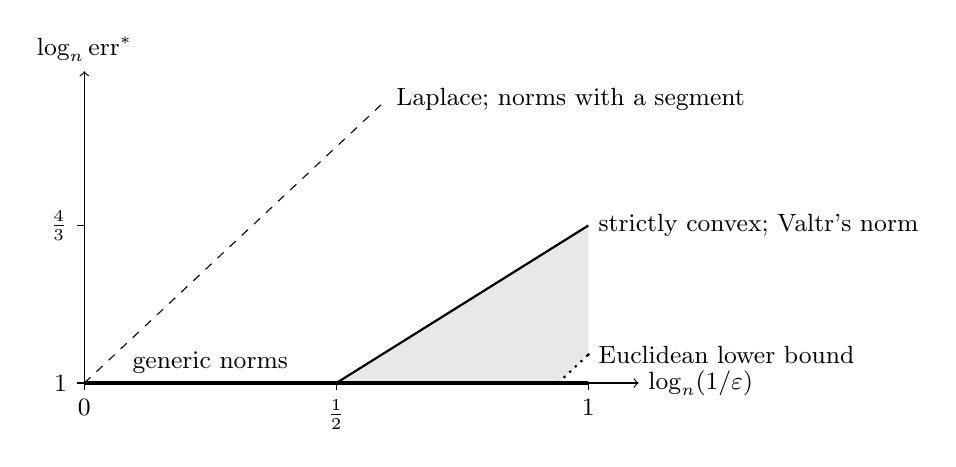
\begin{tikzpicture}[x=6.4cm,y=6cm]
  % vertical coordinate = exponent minus 1; schematic delta = 0.06
  \fill[gray!18] (0,0) -- (0.5,0) -- (1,0.3333) -- (1,0.06) -- (0.94,0) -- cycle;
  \draw[->] (0,0) -- (1.1,0) node[right] {\small $\log_n(1/\eps)$};
  \draw[->] (0,0) -- (0,0.66) node[above] {\small $\log_n \errs$};
  \draw (0,0) -- (0,-0.015) node[below] {\small $0$};
  \draw (0.5,0) -- (0.5,-0.015) node[below] {\small $\frac12$};
  \draw (1,0) -- (1,-0.015) node[below] {\small $1$};
  \draw (0,0) -- (-0.015,0) node[left] {\small $1$};
  \draw (0,0.3333) -- (-0.015,0.3333) node[left] {\small $\frac43$};
  \draw[dashed] (0,0) -- (0.6,0.6) node[right] {\small Laplace; norms with a segment};
  \draw[thick] (0,0) -- (0.5,0) -- (1,0.3333) node[right] {\small strictly convex; Valtr's norm};
  \draw[thick,dotted] (0.94,0) -- (1,0.06) node[right] {\small Euclidean lower bound};
  \fill (1,0.06) circle (0.6pt);
  \draw[very thick] (0,0) -- (1,0);
  \node[above] at (0.25,0.0) {\small generic norms};
\end{tikzpicture}
\caption{Exponent of the optimal error against $\log_n(1/\eps)$. Shaded: the range allowed for the Euclidean norm by \cref{thm:euclid}; its lower edge is drawn with $\delta=0.06$, while the best known value is $\delta\ge0.014$.}
\label{fig:rates}
\end{figure}

\subparagraph*{Summary and provenance.}
\Cref{tab:results} lists the results and says which parts are new. We regard the geometric results (\cref{thm:incidences,thm:norms,thm:euclid}) as the main contribution. \Cref{thm:reduction} is the bridge; \cref{sec:privacy} adds an algorithm that does not need to know $\Lam_k$, at a logarithmic cost.

\begin{table}[!t]
\centering\small
\begin{tabular}{@{}lll@{}}
\toprule
Result & Statement & Status \\
\midrule
\Cref{thm:reduction} & $\errs(\eps,n)=\Theta(\Lam_{\lceil1/\eps\rceil}(n))$ & known tools; new form \\
\Cref{thm:incidences} & $\Lam_k(n)$ and $I(n,k)$ agree up to a factor $2$ ($k\le n/2$) & new (short) \\
\Cref{thm:norms}(1),(4) & segment norms; generic norms & new; uses \cite{ABS23} \\
\Cref{thm:norms}(2) & strictly convex norms & known incidence bound \\
\Cref{thm:norms}(3) & Valtr's norm is extremal for every $k$ & new; extends \cite{Valtr05} \\
\Cref{thm:euclid} & Euclidean window; separation iff $u(n)\ge n^{1+\Omega(1)}$ & new connection \\
\Cref{thm:adaptive} & algorithm without knowledge of $\Lam_k$ & known tools \cite{KNRS13,RS16} \\
\bottomrule
\end{tabular}
\caption{Results and their provenance.}
\label{tab:results}
\end{table}

\subparagraph*{Related work.}
\emph{Unit distances and incidences.} Besides the bounds above, the unit-distance problem is surveyed by Brass, Moser and Pach~\cite{BrassMoserPach05}. The $O(n^{4/3})$ bound follows from incidence bounds for points and curves~\cite{SzemerediTrotter83,CEGSW90,PachSharir98}, and Sz\'ekely's crossing-number argument~\cite{Szekely97} gives it for any family of curves in which two curves meet in at most two points and two points lie on at most two curves. For normed planes, Swanepoel's survey~\cite{Swanepoel18} describes the known results, including Valtr's construction. After the disproof of Erd\H{o}s's conjecture~\cite{OpenAI2026,Remarks2026}, Sawin~\cite{Sawin2026} gave the exponent $1.014$ and Emmerich~\cite{Emmerich2026} optimised explicit finite certificates. We use these results only through \cref{thm:incidences}; we do not use their structure.

\emph{Node privacy.} Node differential privacy for graphs was studied by Blocki, Blum, Datta and Sheffet~\cite{BBDS13} and by Kasiviswanathan, Nissim, Raskhodnikova and Smith~\cite{KNRS13}, who introduced the bounded-degree flow statistic we use. For a family closed under deletion, the restricted sensitivity of Blocki, Blum, Datta and Sheffet is $\Lam_1(n)$ in our notation, which leads to error about $\Lam_1(n)/\eps$. \Cref{thm:reduction} replaces this by $\Lam_{\lceil 1/\eps\rceil}(n)$, which is never larger; for strictly convex norms it is smaller by a factor of order at least $\eps^{-2/3}$. Raskhodnikova and Smith~\cite{RS16} developed Lipschitz extensions and the generalized exponential mechanism used in \cref{sec:privacy}. Instance-dependent guarantees in terms of down sensitivity appear in work of Asi and Duchi~\cite{AsiDuchi20}, Fang, Dong and Yi~\cite{FDY22}, and Dong, Fang, Yi, Tao and Machanavajjhala~\cite{R2T22}; see also Cummings and Durfee~\cite{CummingsDurfee20}. Recent node-private results include counting connected components~\cite{KalemajRST23}, continual observation~\cite{JainSmithWagaman24} and graphon estimation~\cite{ChenEtAl24Graphon}. Raskhodnikova, Smith, Wagaman and Zavyalov~\cite{RSWZ26} study node privacy in the \emph{local} model, where each person randomizes their own edge list; we work in the central model, where a trusted curator holds the data. We are not aware of earlier work that links node privacy to incidence geometry.

%======================================================================
\section{Overview of the proofs}
\label{sec:overview}

\subparagraph*{Why the privacy cost is $\Lam_{\lceil 1/\eps\rceil}$.}
The upper bound uses one public threshold. The surrogate $g_D$ of \cite{KNRS13} changes by at most $D$ when a point is added or removed, and it undercounts $U(P)$ by at most the degree tail $\tail_D(P)=\sum_p(\deg_P(p)-D)_+$. Set $k=\lceil1/\eps\rceil$ and $D=\Lam_k(n)/k$. The vertices of degree above $D$ form a set $S$, and $\tail_D(P)\le S_{|S|}(P)-|S|D\le\Lam_{|S|}(n)-|S|D$. The average $\Lam_j(n)/j$ cannot increase with $j$, so this is at most $\Lam_k(n)$ for every value of $|S|$. Laplace noise of scale $D/\eps\le\Lam_k(n)$ completes the bound.

For the lower bound, take a set $P^\star$ with $S_k(P^\star)=\Lam_k(n)$, where now $k\approx 1/\eps$, and remove its $k$ points of largest degree. Re-inserting them one at a time is a path of $k\le1/\eps$ neighbouring inputs along which the count grows by at least $\Lam_k(n)/2$. A private algorithm cannot distinguish the two ends of such a path well, so it errs by $\Omega(\Lam_k(n))$ on one of them.

\subparagraph*{Why $\Lam_k$ is an incidence count.}
If $C$ is the set of $k$ points of largest degree in $P$, then $S_k(P)$ is the number of incidences between $P$ and the unit circles centred at points of $C$. Conversely, given $n$ points and $k$ unit circles, adding the $k$ centres to the point set turns incidences into degrees. Splitting the points into two halves keeps the total size below~$n$ at a loss of a factor~$2$.

\subparagraph*{Why the norms differ.}
If the unit circle contains a segment, two parallel rows of points give a complete bipartite unit-distance graph, so $\Lam_k(n)=\Theta(kn)$. If the norm is strictly convex, two distinct unit circles meet in at most two points and two points lie on at most two unit circles; the crossing-number argument then gives $I(n,k)=O(n^{2/3}k^{2/3}+n+k)$. For Valtr's norm, the upper half of each unit circle is a parabolic arc, and the map $(x,y)\mapsto(x,y+x^2/2)$ sends all these arcs to segments of lines. The standard grid construction for point--line incidences, at the right aspect ratio, then gives an exact count of unit distances (\cref{lem:valtr-grid}) and $\Lam_k(n)=\Omega(n^{2/3}k^{2/3})$ for every $\sqrt n\le k\le n$. For generic norms the bound of~\cite{ABS23} on $u(n)$ caps $\Lam_k(n)\le 2u(n)$.

\subparagraph*{Why the 2026 result enters.}
The averaging bound $\Lam_k(n)\ge 2k\,u(n)/n$ holds because the $k$ largest of $n$ degrees have at least the average degree. With $k=\lceil 1/\eps\rceil$ close to $n$, \cref{thm:reduction} turns a superlinear $u(n)$ into a superlinear privacy cost. Conversely $\Lam_k(n)\le\Lam_n(n)=2u(n)$, so no other source of superlinear cost exists.

%======================================================================
\section{Preliminaries}
\label{sec:prelim}

\subparagraph*{Geometry.}
Fix a norm $\nrm{\cdot}$ on $\R^2$ with unit circle $\mathbb S=\{x:\nrm{x}=1\}$; a \emph{unit circle} is a translate $c+\mathbb S$. For a finite set $P$, $\deg_P(p)$ is the number of $q\in P$ with $\nrm{p-q}=1$, and $U(P)$ is the number of edges of $G(P)$. For a finite family $\Gamma$ of curves, $I(P,\Gamma)$ is the number of pairs $(p,\gamma)\in P\times\Gamma$ with $p\in\gamma$. Since $\mathbb S=-\mathbb S$, a point $p$ lies on $c+\mathbb S$ exactly when $\nrm{p-c}=1$. We write $\cP_n$ for the family of point sets with at most $n$ points. The functions $\Lam_k(n)$ and $I(n,k)$ are non-decreasing in both arguments, and $\Lam_k(n)=\Lam_n(n)=2u(n)$ for $k\ge n$.

\subparagraph*{Node differential privacy, for geometers.}
An \emph{algorithm} $M$ maps each finite point set $P$ to a random real number $M(P)$. Two point sets are \emph{node neighbours} if one is obtained from the other by adding one point. The word ``node'' refers to the graph $G(P)$: adding a point adds a vertex together with all its edges.

\begin{definition}
Let $\eps>0$ and let $\cF$ be a family of finite point sets. An algorithm $M$ is \emph{$\eps$-node-private on $\cF$} if for all node neighbours $P,Q\in\cF$ and every measurable $T\subseteq\R$,
\(
  \Pr[M(P)\in T]\le e^{\eps}\Pr[M(Q)\in T].
\)
\end{definition}

The definition says that the output reveals little about whether any single person is present. Smaller $\eps$ means stronger privacy; the range $\eps\le1$ is the usual one. We use three standard facts~\cite{DMNS06,DworkRoth14}. (i)~\emph{Laplace mechanism:} if $|f(P)-f(Q)|\le\Delta$ for all node neighbours, then $f(P)+Z$ with $Z$ drawn from the Laplace density $\frac{\eps}{2\Delta}e^{-\eps|z|/\Delta}$ is $\eps$-node-private, and $\Ex|Z|=\Delta/\eps$. For $f=U$ one has $\Delta=n-1$, which gives error $(n-1)/\eps$; we call this the \emph{standard Laplace mechanism}. (ii)~\emph{Groups:} if $P$ and $Q$ are joined by a path of $h$ node neighbours in $\cF$, then $\Pr[M(P)\in T]\le e^{h\eps}\Pr[M(Q)\in T]$. (iii)~The following two-point bound, which we prove for completeness.

\begin{lemma}
\label{lem:two-point}
Let $M$ be $\eps$-node-private on $\cF$, and let $P,Q\in\cF$ be joined by a path of $h$ node neighbours in $\cF$ with $h\eps\le1$. If $U(Q)-U(P)=\Delta>0$, then $\Ex|M(P)-U(P)|$ or $\Ex|M(Q)-U(Q)|$ is at least $\Delta/(2(1+e))$.
\end{lemma}

\begin{proof}
Let $\alpha$ be the larger of the two expected errors and $T=[U(P)+\Delta/2,\infty)$. By Markov's inequality $\Pr[M(P)\in T]\le 2\alpha/\Delta$ and $\Pr[M(Q)\notin T]\le2\alpha/\Delta$. By (ii), $1-2\alpha/\Delta\le\Pr[M(Q)\in T]\le e\cdot 2\alpha/\Delta$, so $\alpha\ge\Delta/(2(1+e))$.
\end{proof}

%======================================================================
\section{The reduction}
\label{sec:reduction}

\begin{lemma}
\label{lem:average}
For every $n$, the sequence $k\mapsto\Lam_k(n)/k$ is non-increasing. Hence $\Lam_j(n)\le (j/k)\Lam_k(n)$ for $j\ge k$.
\end{lemma}

\begin{proof}
For a fixed $P$, $S_k(P)/k$ is the average of the $k$ largest degrees (with zero padding), which does not increase when $k$ grows. A pointwise maximum of non-increasing sequences is non-increasing.
\end{proof}

For a graph $G$ and a real number $D\ge0$, let
\[
  g_D(G)=\max\Bigl\{\sum_{e\in E(G)}x_e:\ 0\le x_e\le1,\ \sum_{e\ni v}x_e\le D\ \text{for every vertex }v\Bigr\}.
\]
It equals one half of the maximum-flow value in the network of Kasiviswanathan, Nissim, Raskhodnikova and Smith~\cite{KNRS13} (\cref{prop:flow-lp} in \cref{app:surrogates}). We write $g_D(P)$ for $g_D(G(P))$.

\begin{lemma}
\label{lem:surrogate}
For every real $D\ge0$: (a) if $P,Q$ are node neighbours then $|g_D(P)-g_D(Q)|\le D$; (b) $U(P)-\tail_D(P)\le g_D(P)\le U(P)$ for every $P$.
\end{lemma}

\begin{proof}
(a) Let $Q=P\cup\{q\}$. An optimal solution for $Q$, restricted to the edges not containing $q$, is feasible for $P$ and loses at most $\sum_{e\ni q}x_e\le D$. An optimal solution for $P$, extended by zeros, is feasible for $Q$. (b) The upper bound holds since $x_e\le1$. For the lower bound put $x_e=\min\{1,D/\deg u,D/\deg v\}$ for $e=uv$. At each vertex $v$ the sum is at most $\deg v\cdot\min\{1,D/\deg v\}\le D$. Each edge loses $1-x_e\le(1-D/\deg u)_++(1-D/\deg v)_+$, and summing over edges gives $\sum_v\deg v\,(1-D/\deg v)_+=\tail_D(P)$.
\end{proof}

\begin{lemma}
\label{lem:tail}
For every $P\in\cP_n$ and real $D\ge0$, $\tail_D(P)\le\max_{0\le j\le n}\bigl(\Lam_j(n)-jD\bigr)$, where $\Lam_0=0$.
\end{lemma}

\begin{proof}
Let $S$ be the set of points of degree larger than $D$ and $j=|S|$. Then $\tail_D(P)=\sum_{p\in S}\deg_P(p)-jD\le S_j(P)-jD\le\Lam_j(n)-jD$.
\end{proof}

The proof below uses only properties (a) and (b) of \cref{lem:surrogate}. Any statistic with these two properties can replace $g_D$; for integer $D$ this includes the integral statistic of \cref{app:surrogates}.

\reduction*

\begin{proof}
\emph{Upper bound.} Let $k=\lceil1/\eps\rceil$, $\lambda=\Lam_k(n)$ and $D=\lambda/k$. The algorithm outputs $g_D(P)+Z$ with $Z$ Laplace of scale $D/\eps$; it is $\eps$-node-private on all finite sets by \cref{lem:surrogate}(a). For $j\ge k$, \cref{lem:average} gives $\Lam_j(n)-jD\le0$, and for $j<k$ we have $\Lam_j(n)-jD\le\lambda$. By \cref{lem:tail} and \cref{lem:surrogate}(b), for every $P\in\cP_n$,
\[
  \Ex|g_D(P)+Z-U(P)|\le\tail_D(P)+\Ex|Z|\le\lambda+\frac{\lambda}{k\eps}\le2\lambda .
\]

\emph{Lower bound.} Let $m=\min\{\lfloor1/\eps\rfloor,n\}\ge1$ and choose $P^\star\in\cP_n$ with $S_m(P^\star)=\Lam_m(n)$. Let $C$ consist of $\min\{m,|P^\star|\}$ points of $P^\star$ of largest degree and $P_0=P^\star\setminus C$. Adding the points of $C$ to $P_0$ one at a time gives a path of $|C|\le m$ node neighbours inside $\cP_n$. Every edge counted in $\sum_{c\in C}\deg(c)=\Lam_m(n)$ is counted at most twice, so $U(P^\star)-U(P_0)\ge\Lam_m(n)/2$. Since $m\eps\le1$, \cref{lem:two-point} shows that every $\eps$-node-private algorithm has expected error at least $\Lam_m(n)/(4(1+e))$ on $P_0$ or on $P^\star$. Finally, if $m=n$ then $\Lam_k(n)=\Lam_m(n)$; otherwise $k\le\lfloor1/\eps\rfloor+1\le2m$, and \cref{lem:average} gives $\Lam_k(n)\le2\Lam_m(n)$.

\emph{Other families.} The upper bound used only \cref{lem:surrogate}, which holds for all graphs. The lower bound used only that $P_0$ and the intermediate sets belong to the family. Both hold for any family closed under deleting points and any graph in which adjacency of two points depends only on these two points.
\end{proof}

\begin{remark}
\label{rem:unknown}
The algorithm needs the value $\Lam_k(n)$. If only an upper bound $\lambda\ge\Lam_k(n)$ is known, the same proof with $D=\lambda/k$ gives error at most $2\lambda$. For the Euclidean norm this yields error $O(n+n^{2/3}\eps^{-2/3})$ from \cref{thm:norms}(2). \Cref{thm:adaptive} below removes the need for any bound at a logarithmic cost.
\end{remark}

%======================================================================
\section{Top-degree mass and incidences}
\label{sec:mass}

\incidences*

\begin{proof}
\emph{Lower bounds.} Placing $n-1$ points on the unit circle around a further point gives $S_1\ge n-1$. If $|P|=n$ and $U(P)=u(n)$, the average degree is $2u(n)/n$, and the $k$ largest degrees have at least this average, so $S_k(P)\ge 2k\,u(n)/n$.

\emph{$\Lam_k(n)\le I(n,k)$.} Let $P\in\cP_n$ and let $C$ be a set of $\min\{k,|P|\}$ points of $P$ of largest degree. Then $S_k(P)=\sum_{c\in C}|P\cap(c+\mathbb S)|$. If $|C|<k$, add $k-|C|$ further centres far from $P$; this does not change the count, so $S_k(P)\le I(n,k)$.

\emph{$I(n-k,k)\le\Lam_k(n)$.} Let $B$ have at most $n-k$ points and let $R$ be a set of $k$ centres. The set $Q=B\cup R$ has at most $n$ points, and each $r\in R$ satisfies $\deg_Q(r)\ge|B\cap(r+\mathbb S)|$, because $r\notin r+\mathbb S$. Since $S_k(Q)$ is at least the sum of the degrees of any $k$ points of $Q$, $\Lam_k(n)\ge S_k(Q)\ge\sum_{r\in R}|B\cap(r+\mathbb S)|$.

\emph{$I(n,k)\le2\Lam_k(n)$ for $k\le n/2$.} Let $B$ be a set of at most $n$ points, $R$ a set of $k$ centres, and $\Gamma_R=\{r+\mathbb S\}_{r\in R}$. Split $B$ into two parts of at most $\lceil n/2\rceil$ points each, and let $B'$ be a part with $I(B',\Gamma_R)\ge I(B,\Gamma_R)/2$. Since $|B'|\le\lceil n/2\rceil\le n-k$, the previous paragraph gives $\Lam_k(n)\ge I(B',\Gamma_R)\ge I(B,\Gamma_R)/2$.
\end{proof}

\Cref{lem:tail} also bounds the degree tail of every set by the top-degree mass. With \cref{thm:norms}(2) this gives, for every strictly convex norm,
\begin{equation}
\label{eq:tail}
  \tail_D(P)\le\max_{j}\bigl(C(n^{2/3}j^{2/3}+n)-jD\bigr)=O\bigl(n^2/D^2+n\bigr)\qquad(P\in\cP_n,\ D\ge1).
\end{equation}
Both terms are needed. A star with $2D$ leaves, repeated $\lfloor n/(2D+1)\rfloor$ times, has tail $\Omega(n)$. Since $\tail_D(P)\ge S_k(P)-kD$ for every $k$, \cref{thm:norms}(3) with $k\asymp n^2/D^3$ shows that for Valtr's norm the first term is attained when $n^{1/3}\lesssim D\lesssim n^{1/2}$. We note that \eqref{eq:tail} applies the incidence bound once, to the circles centred at the high-degree points; summing a bound on the number of $j$-rich points over all $j>D$ would lose a logarithmic factor.

%======================================================================
\section{Norms on the plane}
\label{sec:norms}

\norms*

\begin{proof}[Proof of (1)]
Let the segment $\{v+tw:|t|\le1\}$ lie on $\mathbb S$. Put $m=\lfloor n/2\rfloor$, $a_i=(i/m)w$ and $b_j=v+(j/m)w$ for $0\le i,j<m$. Then $b_j-a_i=v+\frac{j-i}{m}w$ lies on the segment, so all $m^2$ pairs $\{a_i,b_j\}$ are at unit distance. (The points are distinct, since a segment on $\mathbb S$ does not lie on a line through the origin.) Every point has degree at least $m$, and $2m\ge n-1$, so $S_k\ge m\min\{k,n-1\}$. The upper bound holds because every degree is at most $n-1$.
\end{proof}

\begin{proof}[Proof of (2)]
In a strictly convex norm, two distinct unit circles meet in at most two points, and two distinct points lie on at most two common unit circles (\cref{lem:pseudo} in \cref{app:geometry}). For such families, Sz\'ekely's crossing-number argument~\cite{Szekely97}, or the theorem of Pach and Sharir~\cite{PachSharir98}, gives $I(P,\Gamma)\le C_0(|P|^{2/3}|\Gamma|^{2/3}+|P|+|\Gamma|)$; we include the argument in \cref{app:geometry}. By \cref{thm:incidences}, $\Lam_k(n)\le I(n,k)\le C_0(n^{2/3}k^{2/3}+n+k)$, and $k\le n$.
\end{proof}


\begin{figure}[!t]
\centering
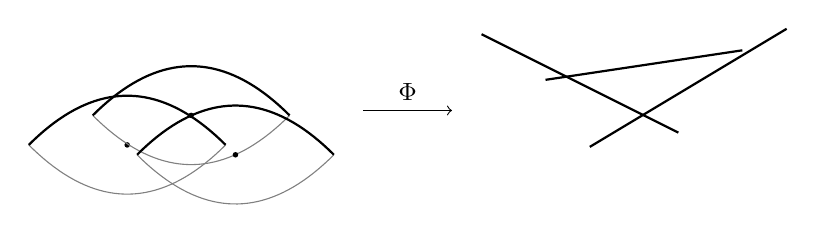
\begin{tikzpicture}[scale=1.25]
  \foreach \a/\b in {-0.5/0, 0.15/0.3, 0.6/-0.1} {
    \draw[gray] plot[domain=-1:1,samples=40] ({\a+\x},{\b-0.5*(1-\x*\x)});
    \draw[thick] plot[domain=-1:1,samples=40] ({\a+\x},{\b+0.5*(1-\x*\x)});
    \fill (\a,\b) circle (0.8pt);
  }
  \draw[->] (1.9,0.35) -- node[above] {\small $\Phi$} (2.8,0.35);
  \begin{scope}[xshift=4.6cm]
    \foreach \a/\b in {-0.5/0, 0.15/0.3, 0.6/-0.1} {
      \draw[thick] ({\a-1},{\b+0.5-0.5*\a*\a+\a*(\a-1)}) -- ({\a+1},{\b+0.5-0.5*\a*\a+\a*(\a+1)});
    }
  \end{scope}
\end{tikzpicture}
\caption{Left: three unit circles of Valtr's norm, each bounded by two parabolic arcs. Right: the map $\Phi(x,y)=(x,y+x^2/2)$ sends the upper arcs (bold) to line segments whose slope is the first coordinate of the centre. Point sets with many point--line incidences therefore yield many unit distances (\cref{lem:valtr-grid}).}
\label{fig:valtr}
\end{figure}

\begin{lemma}[Valtr grid]
\label{lem:valtr-grid}
Let $A,B\ge1$ be integers. For $1\le i\le A$, $1\le j\le 2AB$, $1\le s\le B$ and $1\le t\le AB$ put
\[
  p_{ij}=\Bigl(\frac{i}{2A},\ \frac{j}{4AB}-\frac{i^2}{8A^2}\Bigr),
  \qquad
  c_{st}=\Bigl(\frac{s}{2B},\ \frac{t}{4AB}-\frac12+\frac{s^2}{8B^2}\Bigr).
\]
The $2A^2B$ points $p_{ij}$ are distinct, the $AB^2$ centres $c_{st}$ are distinct, no point equals a centre, and $\nrm{p_{ij}-c_{st}}_V=1$ holds if and only if $j=si+t$. In particular, exactly $A^2B^2$ point--centre pairs are at unit distance.
\end{lemma}

\begin{proof}
For $d=(d_x,d_y)$ we have $\nrm{d}_V=1$ if and only if $\sqrt{d_x^2+d_y^2}=1-|d_y|$, that is, if and only if $d_x^2=1-2|d_y|$. Every point has second coordinate at least $\frac1{4AB}-\frac18>-\frac18$, and every centre has second coordinate at most $\frac14-\frac12+\frac18=-\frac18$. Hence no point equals a centre, and for $d=p_{ij}-c_{st}$ we have $d_y>0$. Write $x=\frac{i}{2A}$ and $a=\frac{s}{2B}$. Then $1-2d_y=x^2+a^2-\frac{2j}{4AB}+\frac{2t}{4AB}$ and $d_x^2=x^2-2ax+a^2$, so $\nrm{d}_V=1$ if and only if $\frac{j}{4AB}=ax+\frac{t}{4AB}$, that is, $j=si+t$. For each of the $AB^2$ pairs $(s,t)$ and each $i\le A$, the value $si+t$ lies in $[2,2AB]$, so it is a valid index $j$. This gives exactly $A\cdot AB^2$ pairs. Distinctness is clear from the coordinates.
\end{proof}

In terms of \cref{fig:valtr}: the map $\Phi$ sends $p_{ij}$ to the grid point $(\frac{i}{2A},\frac{j}{4AB})$ and the upper arc of $c_{st}+\mathbb S$ into the line of slope $\frac{s}{2B}$ and intercept $\frac{t}{4AB}$, so the lemma is the standard grid example for point--line incidences~\cite{SzemerediTrotter83}. The lower arcs carry no incidences, since every point lies above every centre.

\begin{proof}[Proof of (3)]
The norm $\nrm{\cdot}_V$ is the sum of the Euclidean norm and the seminorm $|y|$, so it is strictly convex. Let $m=\lfloor n/2\rfloor$. If $\sqrt n\le k\le m$, choose $A,B\ge1$ with $2A^2B\le m$, $AB^2\le k$ and $A^2B^2\ge n^{2/3}k^{2/3}/53$ (\cref{app:geometry}). The set $Q$ of all points and centres of \cref{lem:valtr-grid} has at most $m+k\le n$ elements, and $S_k(Q)$ is at least the sum of the degrees of the $AB^2\le k$ centres, which is at least $A^2B^2$. The cases $k<\sqrt n$ (where $\Lam_k(n)\ge n-1$) and $k>m$ (by monotonicity in $k$) are treated in \cref{app:geometry}.
\end{proof}

\begin{proof}[Proof of (4)]
By~\cite{ABS23} with $d=2$, for every norm outside a meagre set and every $n$, every $n$ points span at most $n\log_2 n$ unit distances. Then $\Lam_k(n)\le\Lam_n(n)=2u(n)\le2n\log_2 n$. The lower bound $n-1$ holds in every norm.
\end{proof}

\begin{proof}[Proof of \cref{cor:norms-privacy}]
Let $k=\lceil1/\eps\rceil\le n-1$ and apply \cref{thm:reduction}. With a segment, $\Lam_k(n)\ge\lfloor n/2\rfloor/\eps$, and the standard Laplace mechanism has error $(n-1)/\eps$. For strictly convex norms, (2) gives $2\Lam_k(n)=O(n+n^{2/3}k^{2/3})$ and $k\le 2/\eps$; (3) gives the matching lower bound for Valtr's norm. For generic norms, \cref{thm:reduction} and (4) give $(n-1)/(8(1+e))\le\errs(\eps,n)\le2\Lam_k(n)\le4n\log_2n$ for every $\eps\in(0,1]$.
\end{proof}

\euclid*

\begin{proof}
Let $k=\lceil1/\eps\rceil$, so $1/\eps\le k\le\min\{n,2/\eps\}$. By \cref{thm:reduction,thm:incidences}, $\errs(\eps,n)\ge\frac{1}{8(1+e)}\max\{n-1,2u(n)/(\eps n)\}$. The upper bound follows from \cref{thm:reduction,thm:norms}(2). For $\eps\ge n^{-1/2}$ we have $n^{2/3}\eps^{-2/3}\le n$.

For the equivalence, if $u(n)\ge n^{1+\delta}$ then at $\eps=1/n$ the lower bound is at least $c\,u(n)\ge c\,n^{1+\delta}$, which exceeds $n^{1+\delta/2}$ for large~$n$. Conversely, $\errs(\eps,n)\le2\Lam_k(n)\le2\Lam_n(n)=4u(n)$ for every $\eps$, so a lower bound $n^{1+\delta'}$ on the error forces $u(n)\ge n^{1+\delta'}/4$. Finally, Sawin~\cite{Sawin2026} gives $u(n)>n^{1.014}$ for infinitely many $n$; for these $n$ and $\eps=n^{-1+\eta}$ the lower bound is at least $c\,n^{-\eta}u(n)\ge c\,n^{1.014-\eta}$. The comparison with generic norms is \cref{cor:norms-privacy}.
\end{proof}

\subparagraph*{What the separation does and does not say.}
The separation in \cref{thm:euclid} appears only for $\eps\le n^{-1+0.014}$, that is, for very strong privacy. At such $\eps$ the optimal error is already comparable to the count itself, so we do not see it as a recommendation for practice. Its content is structural: the shape of the Euclidean rate curve near $\eps=1/n$ is decided exactly by whether $u(n)$ is polynomially superlinear, and the 2026 results settle this. For larger $\eps$ the curve is decided by $I(n,k)$ with $k<n$, where the gap in \cref{thm:euclid} is open.

%======================================================================
\section{Algorithms and other distance graphs}
\label{sec:privacy}

\subparagraph*{An algorithm that does not need $\Lam_k$.}
The algorithm of \cref{thm:reduction} uses the unknown number $\Lam_k(n)$. The following result, which combines the surrogate of~\cite{KNRS13} with the generalized exponential mechanism of Raskhodnikova and Smith~\cite{RS16}, adapts to the input instead. It is not new as a method; we include it because its guarantee has a direct geometric reading.

\begin{theorem}
\label{thm:adaptive}
Let $K=1+\lceil\log_2 n\rceil$. There is an $\eps$-node-private algorithm such that for every $P\in\cP_n$ and $\beta\in(0,\frac12)$, with probability at least $1-\beta$, its error is $O(S_t(P)+t)$ with $t=\lceil\log(K/\beta)/\eps\rceil$. Consequently the error is $O\bigl(\log(K/\beta)\,(\Lam_{\lceil1/\eps\rceil}(n)+1/\eps)\bigr)$.
\end{theorem}

The algorithm selects a threshold $D$ from $\{1,2,4,\dots,2^{K-1}\}$ privately and then releases $g_D(P)$ with Laplace noise; the proof is in \cref{app:adaptive}. The bound $S_t(P)$ is the number of incidences between $P$ and the $t$ richest unit circles centred in~$P$. For instance, if every point of $P$ has degree at most $\Delta$, the error is $O(\Delta\log(K/\beta)/\eps)$ regardless of~$n$.

\subparagraph*{Surrogates.}
\Cref{thm:reduction} needs real thresholds, because $\Lam_k(n)/k$ need not be an integer; this is one reason to use the fractional statistic $g_D$. The integral statistic $f_D(G)$, the maximum number of edges of a subgraph of maximum degree at most $D$, satisfies the same two properties for integer $D$ and can be computed by $b$-matching~\cite{Schrijver03,Gabow18}. With $D$ rounded up it gives \cref{thm:reduction} up to an additive $1/\eps$ (\cref{app:surrogates}). Both statistics are computable in polynomial time from $G(P)$.

\subparagraph*{Other distance graphs.}
\Cref{thm:reduction} applies to every family of point sets that is closed under deleting points. Two examples are worked out in \cref{app:regimes}. If the points lie on a grid $\frac1q\Z^2$ and the target distance $r$ satisfies $qr\in\Z$, every degree is at most the number $\Delta$ of representations of $(qr)^2$ as a sum of two squares, and the error is $\Theta(\Delta/\eps)$ whenever $n\ge\lceil 1/\eps\rceil(\Delta+1)$. If the points are $\delta$-separated and adjacency means a distance in $[r-t,r+t]$, every degree is $O((t+\delta)(r+t+\delta)/\delta^2)$; in this case releasing $g_D$ for $D$ equal to this bound is private on all inputs and exact on separated inputs. Finally, \cref{app:promise} treats a class of point sets defined by an upper bound on the number of $j$-rich points for every $j$; this class is not closed under deletion, so \cref{thm:reduction} does not apply, and we give separate matching bounds.

%======================================================================
\section{Open problems}
\label{sec:open}

\subparagraph*{The Euclidean window.}
For $\alpha\in[\frac12,1]$ let $\gamma(\alpha)=\limsup_{n\to\infty}\log\Lam_{\lceil n^{\alpha}\rceil}(n)/\log n$ for the Euclidean norm, and let $1+\delta^\star=\gamma(1)$ be the unit-distance exponent. \Cref{thm:incidences,thm:norms} give
\[
  \max\{1,\ \alpha+\delta^\star\}\;\le\;\gamma(\alpha)\;\le\;\tfrac{2+2\alpha}{3},
\]
with $\delta^\star\ge0.014$, and for Valtr's norm the upper bound is attained. Is the lower bound the truth? In words: can a few unit circles be much richer than average while the unit-distance graph as a whole stays sparse? By \cref{thm:incidences} this is a question about incidences between $n$ points and $k$ unit circles. We are not aware of results on this unbalanced version beyond the bounds above.

\subparagraph*{Instance-wise bounds.}
\Cref{thm:reduction} concerns the worst case over $\cP_n$. A local version would compare an algorithm, at each input $P$, with the best algorithm on a small neighbourhood of $P$. Deleting points is controlled by $S_t(P)$, as in \cref{thm:adaptive}; adding points brings in the external quantity $\max_{c\notin P}|P\cap(c+\mathbb S)|$ and its analogues for several inserted points.

\subparagraph*{Higher dimensions.}
In $\R^3$, $u(n)$ lies between $n^{4/3}\log\log n$~\cite{BrassMoserPach05} and $n^{295/197+o(1)}$~\cite{Zahl19}, so the window is wider and both ends are open. In $\R^d$ with $d\ge4$, points on two orthogonal circles of radius $1/\sqrt2$ form a complete bipartite unit-distance graph, as in \cref{thm:norms}(1), and the standard Laplace mechanism is optimal.

\subparagraph*{Use of generative AI.}
A generative AI assistant (Claude, Anthropic) was used to draft the text and \LaTeX{} source of this version, to propose and check proof arguments, and to run numerical sanity checks of \cref{lem:surrogate,lem:valtr-grid}. Parts of the appendix are adapted from an earlier draft whose language was edited with OpenAI Codex. \textcolor{red}{[Authors: state the extent of human review here, e.g.\ that all statements and proofs were verified and the text rewritten by the authors, who take full responsibility for the content.]}

%======================================================================
\bibliography{refs}

%======================================================================
\appendix
\clearpage
\section*{Appendix}
\addcontentsline{toc}{section}{Appendix}

\section{Surrogate statistics}
\label{app:surrogates}

\subparagraph*{The flow statistic.}
Kasiviswanathan, Nissim, Raskhodnikova and Smith~\cite{KNRS13} define the following network for a graph $G=(V,E)$ and a capacity $D\ge0$. Take a source, a sink, and two copies $v_\ell,v_r$ of each vertex. Add arcs of capacity $D$ from the source to each $v_\ell$ and from each $v_r$ to the sink, and for each edge $uv$ add arcs $(u_\ell,v_r)$ and $(v_\ell,u_r)$ of capacity~$1$. Let $\phi_D(G)$ be the maximum flow value. The definition makes sense for real~$D$.

\begin{proposition}
\label{prop:flow-lp}
For every graph $G$ and real $D\ge0$, $\phi_D(G)/2=g_D(G)$.
\end{proposition}

\begin{proof}
Given a feasible $x$ for $g_D$, send $x_{uv}$ units along both arcs of each edge. This is a feasible flow of value $2\sum_ex_e$. Conversely, from a feasible flow $y$ set $x_{uv}=(y_{u_\ell v_r}+y_{v_\ell u_r})/2$. Then $0\le x_e\le1$, and $\sum_{e\ni v}x_e$ is half the flow through $v_\ell$ plus half the flow through $v_r$, which is at most~$D$. The objective is half the flow value.
\end{proof}

Hence \cref{lem:surrogate} is a property of the statistic of~\cite{KNRS13}; our only additions are the explicit fractional solution in part~(b), which gives the bias bound for every real $D$, and the remark that real thresholds are needed in \cref{thm:reduction}.

\subparagraph*{The integral statistic.}
For an integer $D\ge0$ let $f_D(G)$ be the maximum number of edges in a subgraph of $G$ with maximum degree at most $D$.

\begin{proposition}
\label{prop:integral}
For integer $D\ge0$: (a) $|f_D(G)-f_D(G-v)|\le D$; (b) $|E|-\tail_D(G)\le f_D(G)\le g_D(G)\le|E|$, and both inner inequalities can be strict; (c) $f_D$ and $g_D$ can be computed in polynomial time.
\end{proposition}

\begin{proof}
(a) An optimal subgraph for $G$ has at most $D$ edges at $v$; removing them gives a feasible subgraph of $G-v$. Every feasible subgraph of $G-v$ is feasible for $G$. (b) Repeatedly delete an edge at a vertex of current degree above $D$; each deletion lowers $\sum_v(\deg v-D)_+$ by at least one, so at most $\tail_D(G)$ edges are deleted. Integral solutions are feasible for $g_D$. For a triangle and $D=1$, $f_1=1<3/2=g_1$; for a star with more than $D$ leaves, $g_D=D<|E|$. (c) $g_D$ is a maximum flow; $f_D$ is a maximum-cardinality simple $b$-matching with $b\equiv D$~\cite{Schrijver03,Gabow18}.
\end{proof}

With $D'=\lceil\Lam_k(n)/k\rceil$ in place of $D$ in the proof of \cref{thm:reduction}, the bias is at most $\tail_{D'}\le\tail_{D}\le\Lam_k(n)$ and the noise is at most $(D+1)/\eps\le\Lam_k(n)+1/\eps$, so $f_{D'}$ gives error at most $2\Lam_k(n)+1/\eps$.

%----------------------------------------------------------------------
\section{The adaptive algorithm}
\label{app:adaptive}

In this appendix $\log$ is the natural logarithm. Let $\mathcal D=\{1,2,4,\dots,2^{K-1}\}$ with $K=1+\lceil\log_2 n\rceil$, so $\max\mathcal D\ge n-1$. Fix $\beta\in(0,\frac12)$, split $\eps=\eps_1+\eps_2$ with $\eps_1=\eps_2=\eps/2$, and let $a=\log(2/\beta)$.

\subparagraph*{The selection tool.} The generalized exponential mechanism~\cite{RS16} of Raskhodnikova and Smith takes $K$ candidates with score functions $q_1,\dots,q_K$, which are to be minimized; $q_i$ has sensitivity at most $\Delta_i$. The mechanism is $\eps'$-differentially private, and for every $\beta'\in(0,1)$, with probability at least $1-\beta'$ its output $\hat\imath$ satisfies
\[
  q_{\hat\imath}\le\min_i\bigl(q_i+4\Delta_i\log(K/\beta')/\eps'\bigr).
\]
We use only this guarantee.

\subparagraph*{Algorithm.} Run the generalized exponential mechanism with privacy parameter $\eps_1$ on the scores $q_D(P)=-g_D(P)+aD/\eps_2$, $D\in\mathcal D$, where score $q_D$ is declared to have sensitivity $D$; let $\widehat D$ be the output. Release $g_{\widehat D}(P)+Z$ with $Z$ Laplace of scale $\widehat D/\eps_2$.

\begin{lemma}
\label{lem:adaptive-oracle}
The algorithm is $\eps$-node-private. With probability at least $1-\beta$ its error is at most $\min_{D\in\mathcal D}\{\tail_D(P)+aD/\eps_2+4D\log(2K/\beta)/\eps_1\}$.
\end{lemma}

\begin{proof}
Each score $q_D$ has sensitivity at most $D$ by \cref{lem:surrogate}(a), since $aD/\eps_2$ does not depend on $P$. The selection step is $\eps_1$-node-private by the guarantee above, the release step is $\eps_2$-node-private given $\widehat D$, and the composition is $\eps$-node-private. By the guarantee above with $\beta'=\beta/2$, with probability at least $1-\beta/2$, $q_{\widehat D}(P)\le\min_D\{q_D(P)+4D\log(2K/\beta)/\eps_1\}$. With probability at least $1-\beta/2$, $|Z|\le a\widehat D/\eps_2$. On both events,
\[
  |g_{\widehat D}(P)+Z-U(P)|\le U(P)-g_{\widehat D}(P)+a\widehat D/\eps_2=U(P)+q_{\widehat D}(P),
\]
and $U(P)+q_D(P)\le\tail_D(P)+aD/\eps_2$ by \cref{lem:surrogate}(b).
\end{proof}

\begin{lemma}
\label{lem:oracle-identity}
Let $d_{(1)}\ge d_{(2)}\ge\cdots$ be the degrees of $G(P)$, padded with zeros. For every integer $t\ge1$, $\min_{D\ge0}\{\tail_D(P)+tD\}=S_t(P)$, and $\min_{D\in\mathcal D}\{\tail_D(P)+tD\}\le2S_t(P)+t$.
\end{lemma}

\begin{proof}
For every $D\ge0$, $\tail_D(P)+tD\ge\sum_{i\le t}(d_{(i)}-D)+tD=S_t(P)$, with equality at $D=d_{(t+1)}$. For the grid, if $d_{(t+1)}=0$ take $D=1$: only the top $t$ points have positive degree, so $\tail_1(P)\le S_t(P)$. Otherwise take $D\in\mathcal D$ with $d_{(t+1)}\le D\le2d_{(t+1)}$; then $\tail_D(P)+tD\le S_t(P)-t\,d_{(t+1)}+2t\,d_{(t+1)}\le2S_t(P)$.
\end{proof}

\begin{proof}[Proof of \cref{thm:adaptive}]
By \cref{lem:adaptive-oracle}, the error is at most $\min_{D\in\mathcal D}\{\tail_D(P)+t'D\}$, where $t'=\lceil 2a/\eps+8\log(2K/\beta)/\eps\rceil=O(t)$. By \cref{lem:oracle-identity} this is at most $2S_{t'}(P)+t'$, and $S_{t'}(P)\le\lceil t'/t\rceil S_t(P)$ because $S_j(P)/j$ is non-increasing in $j$. Hence the error is $O(S_t(P)+t)$. For the second statement let $k=\lceil1/\eps\rceil$. Then $S_t(P)\le\Lam_{\max\{t,k\}}(n)\le(t/k+1)\Lam_k(n)$ by \cref{lem:average}, and $t/k\le\log(K/\beta)+1$.
\end{proof}

%----------------------------------------------------------------------
\section{Deferred geometric proofs}
\label{app:geometry}

\begin{lemma}
\label{lem:pseudo}
Let $\mathbb S$ be the unit circle of a strictly convex norm. Two distinct translates of $\mathbb S$ meet in at most two points, and two distinct points lie on at most two common translates of~$\mathbb S$.
\end{lemma}

\begin{proof}
Let $K$ be the unit ball and $v\ne0$. Choose coordinates $(s,\tau)$ with $\tau$ measured along $v$. Each line $\{s=s_0\}$ that meets the interior of $K$ meets $K$ in a segment $[\tau_-(s_0),\tau_+(s_0)]$, where $\tau_-$ is convex and $\tau_+$ is concave; at the two extreme values of $s$ the intersection is a single point, by strict convexity. The boundary of $K+v$ on the same line is $\{\tau_-(s_0)+|v|,\tau_+(s_0)+|v|\}$. Since $\tau_-\le\tau_+$ and $|v|>0$, a common boundary point must satisfy $\tau_+(s_0)=\tau_-(s_0)+|v|$, that is, $h(s_0)=|v|$ for $h=\tau_+-\tau_-$. Strict convexity of $K$ means that the graphs of $\tau_\pm$ contain no segment, so $h$ is strictly concave, and it vanishes at the extreme values of~$s$. A strictly concave function takes a positive value at most twice, which proves the first claim. For the second, $p,q\in c+\mathbb S$ means $c\in(p+\mathbb S)\cap(q+\mathbb S)$ because $\mathbb S=-\mathbb S$, and these two translates are distinct.
\end{proof}

\begin{lemma}
\label{lem:incidence}
There is an absolute constant $C_0$ such that for every strictly convex norm, every finite set $P$ and every finite family $\Gamma$ of distinct unit circles, $I(P,\Gamma)\le C_0(|P|^{2/3}|\Gamma|^{2/3}+|P|+|\Gamma|)$.
\end{lemma}

\begin{proof}
This is the argument of Sz\'ekely~\cite{Szekely97}. Let $N=|P|$ and $m=|\Gamma|$. Draw a multigraph $H$ on $P$: for every $\gamma\in\Gamma$ containing $j\ge2$ points of $P$, join consecutive points along $\gamma$ by the $j$ arcs between them. Then $H$ has at least $I(P,\Gamma)-m$ edges. By \cref{lem:pseudo}, two points are joined by arcs of at most two circles, and each circle contributes at most two such arcs, so every edge has multiplicity at most~$4$. Two arcs of the same circle do not cross, and two circles meet in at most two points, so the drawing has at most $m^2$ crossings. The crossing lemma for multigraphs with bounded multiplicity~\cite{Szekely97} states that a multigraph with $N$ vertices, $e$ edges and multiplicity at most $\mu$ has crossing number at least $c_1e^3/(\mu N^2)$ whenever $e\ge c_2\mu N$, for absolute constants $c_1,c_2>0$. Hence either $I(P,\Gamma)-m<4c_2N$ or $m^2\ge c_1(I(P,\Gamma)-m)^3/(4N^2)$, and in both cases the claim follows.
\end{proof}

\begin{proof}[Completion of the proof of \cref{thm:norms}(3)]
Let $n\ge8$ and $m=\lfloor n/2\rfloor\ge4$, so $n/3\le m$ and $\sqrt n\le m$.

\emph{Case $\sqrt n\le k\le m$.} Put $A_0=(m/2)^{2/3}k^{-1/3}$ and $B_0=k^{2/3}(m/2)^{-1/3}$, so that $2A_0^2B_0=m$ and $A_0B_0^2=k$. Since $k\le m$ and $m\ge4$ we have $(m/2)^2\ge m\ge k$, so $A_0\ge1$; since $k^2\ge n\ge m/2$ we have $B_0\ge1$. Let $A=\lfloor A_0\rfloor\ge A_0/2$ and $B=\lfloor B_0\rfloor\ge B_0/2$. Then $2A^2B\le m$, $AB^2\le k$, and $A^2B^2\ge A_0^2B_0^2/16=(mk/2)^{2/3}/16\ge(nk/6)^{2/3}/16\ge n^{2/3}k^{2/3}/53$. Let $Q$ be the union of the $2A^2B$ points and the $AB^2$ centres of \cref{lem:valtr-grid}; it has at most $m+k\le n$ elements. The $AB^2\le k$ centres have total degree in $G(Q)$ at least $A^2B^2$, so $\Lam_k(n)\ge S_k(Q)\ge n^{2/3}k^{2/3}/53$.

\emph{Case $m<k\le n$.} By monotonicity in $k$ and the previous case with $k=m$, $\Lam_k(n)\ge\Lam_m(n)\ge n^{2/3}m^{2/3}/53\ge n^{2/3}k^{2/3}/111$, since $m\ge n/3\ge k/3$.

\emph{Case $k<\sqrt n$.} Here $\Lam_k(n)\ge n-1\ge n/2\ge n^{2/3}k^{2/3}/2$.

In all cases $\Lam_k(n)\ge\max\{n^{2/3}k^{2/3}/111,\ n/2\}\ge(n^{2/3}k^{2/3}+n)/222$, so (3) holds with $c=1/222$.
\end{proof}

%----------------------------------------------------------------------
\section{A class defined by rich points}
\label{app:promise}

In this appendix the norm is Euclidean. For $j\ge1$ let $R_j(P)$ be the number of points of $P$ of degree at least~$j$. For $C\ge1$ and $D_0\ge1$, call $P$ \emph{$(C,D_0)$-regular} if $R_j(P)\le C|P|^2/j^3$ for every integer $j>D_0$. Deleting a point can violate this condition, so the class is not closed under deletion, and \cref{thm:reduction} does not apply. The bound $R_j(P)=O(n^2/j^3+n/j)$ holds for every set by the incidence bound, so the condition removes exactly the term $n/j$ coming from many stars of degree about~$j$.

\begin{proposition}
\label{prop:promise-upper}
If $P$ is $(C,D_0)$-regular, $|P|=n$, and $D\ge D_0$ is an integer, then $\tail_D(P)=\sum_{j>D}R_j(P)=O(Cn^2/D^2)$. Hence the algorithm $g_D(P)+\Lap(D/\eps)$ with $D\asymp(C\eps n^2)^{1/3}\ge D_0$ has expected error $O(C^{1/3}n^{2/3}\eps^{-2/3})$, and the algorithm of \cref{thm:adaptive} has error $O(C^{1/3}n^{2/3}(\log(K/\beta)/\eps)^{2/3})$ with probability $1-\beta$ whenever $D_0\le(Cn^2\eps/\log(K/\beta))^{1/3}$.
\end{proposition}

\begin{proof}
$\tail_D(P)=\sum_{j>D}R_j(P)\le Cn^2\sum_{j>D}j^{-3}=O(Cn^2/D^2)$. The first algorithm is private on all inputs by \cref{lem:surrogate}(a), and its error is $O(D/\eps+Cn^2/D^2)$. For the second, \cref{lem:adaptive-oracle} bounds the error by $O(\min_{D\in\mathcal D,D\ge D_0}\{Cn^2/D^2+D\log(K/\beta)/\eps\})$; optimise over~$D$.
\end{proof}

\begin{proposition}
\label{prop:promise-lower}
There are absolute constants $a,b>0$ and $n_0$ such that for $n\ge n_0$, $1\le C\le n$, $D_0\ge1$ and $aC^{1/2}n^{-1/2}\le\eps\le1$, every $\eps$-node-private algorithm has expected error at least $b\,C^{1/3}n^{2/3}\eps^{-2/3}$ on some $(C,D_0)$-regular set of at most $n$ points.
\end{proposition}

\begin{proof}
Let $h=\max\{1,\lfloor1/(4\eps)\rfloor\}$, so $1/(8\eps)\le h\le1/\eps$. Choose $a$ large and $\alpha\le\frac12$ small with $2\alpha a^{-2/3}\le\frac12$, and set $L=\lfloor\alpha(Cn^2/h)^{1/3}\rfloor$. Since $(Cn^2/h)^{1/3}\ge(Cn^2\eps)^{1/3}\ge a^{1/3}C^{1/2}n^{1/2}$, for $n\ge n_0$ we get $L\ge\frac\alpha2(Cn^2/h)^{1/3}\ge2$ and $h(L+1)\le2\alpha C^{1/3}n^{2/3}\eps^{-2/3}\le n/2$.
Take $h$ far-apart gadgets, each consisting of a potential centre $c_i$ and $L$ points on its unit circle, with angles chosen so that no two of these $L$ points are at unit distance, together with $n-h(L+1)$ isolated padding points. Let $P_i$ contain all non-centre points and $c_1,\dots,c_i$. Then $|P_h|=n$, $|P_i|\ge n/2$, consecutive sets are node neighbours, and $U(P_h)-U(P_0)=hL$. For $2\le j\le L$ the points of degree at least $j$ are the inserted centres, so $R_j(P_i)\le h\le C|P_i|^2/L^3\le C|P_i|^2/j^3$ by the choice of $\alpha$, and $R_j(P_i)=0$ for $j>L$. Thus every $P_i$ is $(C,D_0)$-regular. Since $h\eps\le1$, \cref{lem:two-point} gives error at least $hL/(2(1+e))=\Omega(C^{1/3}n^{2/3}h^{2/3})=\Omega(C^{1/3}n^{2/3}\eps^{-2/3})$.
\end{proof}

The class is useful as a conditional statement: it describes inputs on which the rich points are spread over many degree levels. We do not know a natural family of point sets with many unit distances that satisfies the condition and is not built from stars, and we leave this as a question.

%----------------------------------------------------------------------
\section{Grid points and separated sets}
\label{app:regimes}

\subparagraph*{Grid points.}
Let $P\subset\frac1q\Z^2$ and let the target distance $r$ satisfy $qr\in\Z$. Points of $\frac1q\Z^2$ at distance $r$ from a grid point correspond to integer solutions of $x^2+y^2=(qr)^2$, so every degree is at most $\Delta=r_2((qr)^2)$, the number of such representations, and $\Delta\le(qr)^{O(1/\log\log(qr))}$~\cite{HardyWright08}. Grid point sets form a family closed under deletion, with $\Lam_k\le k\Delta$. A lattice point together with the $\Delta$ grid points on its circle shows $\Lam_k\ge k\Delta$ when $n\ge k(\Delta+1)$ (use $k$ far-apart copies). By \cref{thm:reduction} the error is $\Theta(\Delta/\eps)$ when $n\ge\lceil1/\eps\rceil(\Delta+1)$; the Laplace mechanism applied to $U$ itself achieves the upper bound. If arbitrary inputs are first rounded to a fixed public grid, neighbours are mapped to equal or neighbouring grid sets, so the rounded statistic inherits privacy.

\subparagraph*{Separated sets and annuli.}
Fix $\delta>0$, $r>0$, $t\ge0$, and let two points be adjacent when their distance lies in $[r-t,r+t]$. Consider the family of $\delta$-separated sets, in which every two points have distance at least~$\delta$; it is closed under deletion. The disks of radius $\delta/2$ around the neighbours of a point $p$ are disjoint and lie in the annulus around $p$ with radii $\max\{0,r-t-\delta/2\}$ and $r+t+\delta/2$. If the inner radius is positive, this annulus has area $2\pi r(2t+\delta)$; otherwise $r\le t+\delta/2$ and the area is at most $\pi(2t+\delta)^2$. In both cases the area is at most $\pi(2t+\delta)(2r+2t+\delta)$, so every degree is at most
\[
  \Delta_{\rm sep}=\frac{4(2t+\delta)(2r+2t+\delta)}{\delta^2}=O\Bigl(\frac{rt+t^2}{\delta^2}+\frac{r+t}{\delta}+1\Bigr).
\]
For $t\le r$ this is $O(rt/\delta^2+r/\delta+1)$. For $t>r$ the term $t^2/\delta^2$ cannot be dropped: then every point within distance $r+t$ of $p$ is a neighbour of $p$, and a disk of radius $t\ge\delta$ contains $\Omega(t^2/\delta^2)$ points of a $\delta$-separated grid. The algorithm $g_D(P)+\Lap(D/\eps)$ with $D=\Delta_{\rm sep}$ is $\eps$-node-private on \emph{all} finite sets by \cref{lem:surrogate}(a); on $\delta$-separated sets every degree is at most $D$, so $g_D(P)=U(P)$ by \cref{lem:surrogate}(b) and the only error is the noise, $\Delta_{\rm sep}/\eps$ in expectation. The same argument applies to threshold graphs (distance at most $r$), with degree $O(r^2/\delta^2+1)$.

\subparagraph*{Several distance bins.}
For a histogram of distances with bins $b_1,\dots,b_L$, adding a point changes all bins at once. A simple private release splits $\eps=\eps_1+\dots+\eps_L$ and runs the one-bin algorithm with parameter $\eps_i$ in bin~$i$.

\end{document}
